\documentclass[1p]{elsarticle_modified}
%\bibliographystyle{elsarticle-num}

%\usepackage[colorlinks]{hyperref}
%\usepackage{abbrmath_seonhwa} %\Abb, \Ascr, \Acal ,\Abf, \Afrak
\usepackage{amsfonts}
\usepackage{amssymb}
\usepackage{amsmath}
\usepackage{amsthm}
\usepackage{scalefnt}
\usepackage{amsbsy}
\usepackage{kotex}
\usepackage{caption}
\usepackage{subfig}
\usepackage{color}
\usepackage{graphicx}
\usepackage{xcolor} %% white, black, red, green, blue, cyan, magenta, yellow
\usepackage{float}
\usepackage{setspace}
\usepackage{hyperref}

\usepackage{tikz}
\usetikzlibrary{arrows}

\usepackage{multirow}
\usepackage{array} % fixed length table
\usepackage{hhline}

%%%%%%%%%%%%%%%%%%%%%
\makeatletter
\renewcommand*\env@matrix[1][\arraystretch]{%
	\edef\arraystretch{#1}%
	\hskip -\arraycolsep
	\let\@ifnextchar\new@ifnextchar
	\array{*\c@MaxMatrixCols c}}
\makeatother %https://tex.stackexchange.com/questions/14071/how-can-i-increase-the-line-spacing-in-a-matrix
%%%%%%%%%%%%%%%

\usepackage[normalem]{ulem}

\newcommand{\msout}[1]{\ifmmode\text{\sout{\ensuremath{#1}}}\else\sout{#1}\fi}
%SOURCE: \msout is \stkout macro in https://tex.stackexchange.com/questions/20609/strikeout-in-math-mode

\newcommand{\cancel}[1]{
	\ifmmode
	{\color{red}\msout{#1}}
	\else
	{\color{red}\sout{#1}}
	\fi
}

\newcommand{\add}[1]{
	{\color{blue}\uwave{#1}}
}

\newcommand{\replace}[2]{
	\ifmmode
	{\color{red}\msout{#1}}{\color{blue}\uwave{#2}}
	\else
	{\color{red}\sout{#1}}{\color{blue}\uwave{#2}}
	\fi
}

\newcommand{\Sol}{\mathcal{S}} %segment
\newcommand{\D}{D} %diagram
\newcommand{\A}{\mathcal{A}} %arc


%%%%%%%%%%%%%%%%%%%%%%%%%%%%%5 test

\def\sl{\operatorname{\textup{SL}}(2,\Cbb)}
\def\psl{\operatorname{\textup{PSL}}(2,\Cbb)}
\def\quan{\mkern 1mu \triangleright \mkern 1mu}

\theoremstyle{definition}
\newtheorem{thm}{Theorem}[section]
\newtheorem{prop}[thm]{Proposition}
\newtheorem{lem}[thm]{Lemma}
\newtheorem{ques}[thm]{Question}
\newtheorem{cor}[thm]{Corollary}
\newtheorem{defn}[thm]{Definition}
\newtheorem{exam}[thm]{Example}
\newtheorem{rmk}[thm]{Remark}
\newtheorem{alg}[thm]{Algorithm}

\newcommand{\I}{\sqrt{-1}}
\begin{document}

%\begin{frontmatter}
%
%\title{Boundary parabolic representations of knots up to 8 crossings}
%
%%% Group authors per affiliation:
%\author{Yunhi Cho} 
%\address{Department of Mathematics, University of Seoul, Seoul, Korea}
%\ead{yhcho@uos.ac.kr}
%
%
%\author{Seonhwa Kim} %\fnref{s_kim}}
%\address{Center for Geometry and Physics, Institute for Basic Science, Pohang, 37673, Korea}
%\ead{ryeona17@ibs.re.kr}
%
%\author{Hyuk Kim}
%\address{Department of Mathematical Sciences, Seoul National University, Seoul 08826, Korea}
%\ead{hyukkim@snu.ac.kr}
%
%\author{Seokbeom Yoon}
%\address{Department of Mathematical Sciences, Seoul National University, Seoul, 08826,  Korea}
%\ead{sbyoon15@snu.ac.kr}
%
%\begin{abstract}
%We find all boundary parabolic representation of knots up to 8 crossings.
%
%\end{abstract}
%\begin{keyword}
%    \MSC[2010] 57M25 
%\end{keyword}
%
%\end{frontmatter}

%\linenumbers
%\tableofcontents
%
\newcommand\colored[1]{\textcolor{white}{\rule[-0.35ex]{0.8em}{1.4ex}}\kern-0.8em\color{red} #1}%
%\newcommand\colored[1]{\textcolor{white}{ #1}\kern-2.17ex	\textcolor{white}{ #1}\kern-1.81ex	\textcolor{white}{ #1}\kern-2.15ex\color{red}#1	}

{\Large $\underline{12a_{0252}~(K12a_{0252})}$}

\setlength{\tabcolsep}{10pt}
\renewcommand{\arraystretch}{1.6}
\vspace{1cm}\begin{tabular}{m{100pt}>{\centering\arraybackslash}m{274pt}}
\multirow{5}{120pt}{
	\centering
	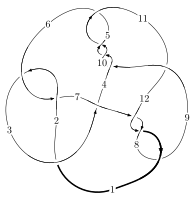
\includegraphics[width=112pt]{../../../GIT/diagram.site/Diagrams/png/1053_12a_0252.png}\\
\ \ \ A knot diagram\footnotemark}&
\allowdisplaybreaks
\textbf{Linearized knot diagam} \\
\cline{2-2}
 &
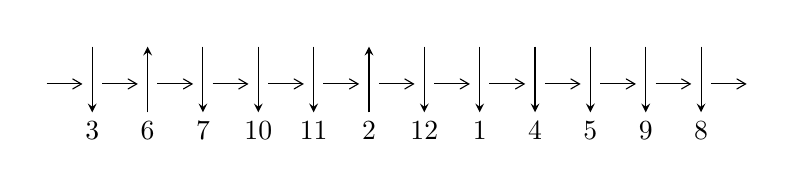
\begin{tikzpicture}[x=20pt, y=17pt]
	% nodes
	\node (C0) at (0, 0) {};
	\node (C1) at (1, 0) {};
	\node (C1U) at (1, +1) {};
	\node (C1D) at (1, -1) {3};

	\node (C2) at (2, 0) {};
	\node (C2U) at (2, +1) {};
	\node (C2D) at (2, -1) {6};

	\node (C3) at (3, 0) {};
	\node (C3U) at (3, +1) {};
	\node (C3D) at (3, -1) {7};

	\node (C4) at (4, 0) {};
	\node (C4U) at (4, +1) {};
	\node (C4D) at (4, -1) {10};

	\node (C5) at (5, 0) {};
	\node (C5U) at (5, +1) {};
	\node (C5D) at (5, -1) {11};

	\node (C6) at (6, 0) {};
	\node (C6U) at (6, +1) {};
	\node (C6D) at (6, -1) {2};

	\node (C7) at (7, 0) {};
	\node (C7U) at (7, +1) {};
	\node (C7D) at (7, -1) {12};

	\node (C8) at (8, 0) {};
	\node (C8U) at (8, +1) {};
	\node (C8D) at (8, -1) {1};

	\node (C9) at (9, 0) {};
	\node (C9U) at (9, +1) {};
	\node (C9D) at (9, -1) {4};

	\node (C10) at (10, 0) {};
	\node (C10U) at (10, +1) {};
	\node (C10D) at (10, -1) {5};

	\node (C11) at (11, 0) {};
	\node (C11U) at (11, +1) {};
	\node (C11D) at (11, -1) {9};

	\node (C12) at (12, 0) {};
	\node (C12U) at (12, +1) {};
	\node (C12D) at (12, -1) {8};
	\node (C13) at (13, 0) {};

	% arrows
	\draw[->,>={angle 60}]
	(C0) edge (C1) (C1) edge (C2) (C2) edge (C3) (C3) edge (C4) (C4) edge (C5) (C5) edge (C6) (C6) edge (C7) (C7) edge (C8) (C8) edge (C9) (C9) edge (C10) (C10) edge (C11) (C11) edge (C12) (C12) edge (C13) ;	\draw[->,>=stealth]
	(C1U) edge (C1D) (C2D) edge (C2U) (C3U) edge (C3D) (C4U) edge (C4D) (C5U) edge (C5D) (C6D) edge (C6U) (C7U) edge (C7D) (C8U) edge (C8D) (C9U) edge (C9D) (C10U) edge (C10D) (C11U) edge (C11D) (C12U) edge (C12D) ;
	\end{tikzpicture} \\
\hhline{~~} \\& 
\textbf{Solving Sequence} \\ \cline{2-2} 
 &
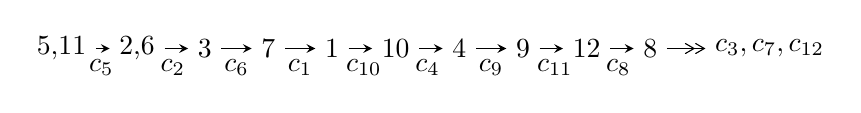
\begin{tikzpicture}[x=23pt, y=7pt]
	% node
	\node (A0) at (-1/8, 0) {5,11};
	\node (A1) at (17/16, 0) {2,6};
	\node (A2) at (17/8, 0) {3};
	\node (A3) at (25/8, 0) {7};
	\node (A4) at (33/8, 0) {1};
	\node (A5) at (41/8, 0) {10};
	\node (A6) at (49/8, 0) {4};
	\node (A7) at (57/8, 0) {9};
	\node (A8) at (65/8, 0) {12};
	\node (A9) at (73/8, 0) {8};
	\node (C1) at (1/2, -1) {$c_{5}$};
	\node (C2) at (13/8, -1) {$c_{2}$};
	\node (C3) at (21/8, -1) {$c_{6}$};
	\node (C4) at (29/8, -1) {$c_{1}$};
	\node (C5) at (37/8, -1) {$c_{10}$};
	\node (C6) at (45/8, -1) {$c_{4}$};
	\node (C7) at (53/8, -1) {$c_{9}$};
	\node (C8) at (61/8, -1) {$c_{11}$};
	\node (C9) at (69/8, -1) {$c_{8}$};
	\node (A10) at (11, 0) {$c_{3},c_{7},c_{12}$};

	% edge
	\draw[->,>=stealth]	
	(A0) edge (A1) (A1) edge (A2) (A2) edge (A3) (A3) edge (A4) (A4) edge (A5) (A5) edge (A6) (A6) edge (A7) (A7) edge (A8) (A8) edge (A9) ;
	\draw[->>,>={angle 60}]	
	(A9) edge (A10);
\end{tikzpicture} \\ 

\end{tabular} \\

\footnotetext{
The image of knot diagram is generated by the software ``\textbf{Draw programme}" developed by Andrew Bartholomew(\url{http://www.layer8.co.uk/maths/draw/index.htm\#Running-draw}), where we modified some parts for our purpose(\url{https://github.com/CATsTAILs/LinksPainter}).
}\phantom \\ \newline 
\centering \textbf{Ideals for irreducible components\footnotemark of $X_{\text{par}}$} 
 
\begin{align*}
I^u_{1}&=\langle 
-3.93238\times10^{36} u^{70}-5.06587\times10^{36} u^{69}+\cdots+5.33198\times10^{36} b+2.44647\times10^{37},\\
\phantom{I^u_{1}}&\phantom{= \langle  }5.07711\times10^{36} u^{70}-1.19436\times10^{37} u^{69}+\cdots+5.33198\times10^{36} a+4.10693\times10^{37},\;u^{71}- u^{70}+\cdots-4 u+4\rangle \\
I^u_{2}&=\langle 
- a u+b+1,\;2 a^2+a u+2 a+2 u+3,\;u^2-2\rangle \\
\\
I^v_{1}&=\langle 
a,\;b+v,\;v^2+v+1\rangle \\
\end{align*}
\raggedright * 3 irreducible components of $\dim_{\mathbb{C}}=0$, with total 77 representations.\\
\footnotetext{All coefficients of polynomials are rational numbers. But the coefficients are sometimes approximated in decimal forms when there is not enough margin.}
\newpage
\renewcommand{\arraystretch}{1}
\centering \section*{I. $I^u_{1}= \langle -3.93\times10^{36} u^{70}-5.07\times10^{36} u^{69}+\cdots+5.33\times10^{36} b+2.45\times10^{37},\;5.08\times10^{36} u^{70}-1.19\times10^{37} u^{69}+\cdots+5.33\times10^{36} a+4.11\times10^{37},\;u^{71}- u^{70}+\cdots-4 u+4 \rangle$}
\flushleft \textbf{(i) Arc colorings}\\
\begin{tabular}{m{7pt} m{180pt} m{7pt} m{180pt} }
\flushright $a_{5}=$&$\begin{pmatrix}1\\0\end{pmatrix}$ \\
\flushright $a_{11}=$&$\begin{pmatrix}0\\u\end{pmatrix}$ \\
\flushright $a_{2}=$&$\begin{pmatrix}-0.952200 u^{70}+2.23999 u^{69}+\cdots+20.1357 u-7.70244\\0.737508 u^{70}+0.950092 u^{69}+\cdots+6.24797 u-4.58829\end{pmatrix}$ \\
\flushright $a_{6}=$&$\begin{pmatrix}1\\u^2\end{pmatrix}$ \\
\flushright $a_{3}=$&$\begin{pmatrix}-0.741052 u^{70}+2.20642 u^{69}+\cdots+17.4237 u-7.13958\\1.16557 u^{70}+1.11369 u^{69}+\cdots+6.11369 u-5.29860\end{pmatrix}$ \\
\flushright $a_{7}=$&$\begin{pmatrix}-1.16962 u^{70}+1.25814 u^{69}+\cdots+8.82584 u-2.37901\\-0.630401 u^{70}-0.239711 u^{69}+\cdots-3.62581 u+2.09462\end{pmatrix}$ \\
\flushright $a_{1}=$&$\begin{pmatrix}-0.429711 u^{70}+0.940016 u^{69}+\cdots+10.0861 u-2.73375\\0.311878 u^{70}-0.164899 u^{69}+\cdots+1.39448 u-0.301335\end{pmatrix}$ \\
\flushright $a_{10}=$&$\begin{pmatrix}u\\u\end{pmatrix}$ \\
\flushright $a_{4}=$&$\begin{pmatrix}- u^2+1\\- u^2\end{pmatrix}$ \\
\flushright $a_{9}=$&$\begin{pmatrix}- u^3+2 u\\- u^3+u\end{pmatrix}$ \\
\flushright $a_{12}=$&$\begin{pmatrix}- u^7+4 u^5-4 u^3\\- u^7+3 u^5-2 u^3+u\end{pmatrix}$ \\
\flushright $a_{8}=$&$\begin{pmatrix}-0.518233 u^{70}+1.13571 u^{69}+\cdots+3.53681 u-1.30370\\-0.0840621 u^{70}+0.422232 u^{69}+\cdots-1.48260 u-0.530560\end{pmatrix}$\\&\end{tabular}
\flushleft \textbf{(ii) Obstruction class $= -1$}\\~\\
\flushleft \textbf{(iii) Cusp Shapes $= 2.34776 u^{70}-2.08944 u^{69}+\cdots-14.6022 u-7.88015$}\\~\\
\newpage\renewcommand{\arraystretch}{1}
\flushleft \textbf{(iv) u-Polynomials at the component}\newline \\
\begin{tabular}{m{50pt}|m{274pt}}
Crossings & \hspace{64pt}u-Polynomials at each crossing \\
\hline $$\begin{aligned}c_{1}\end{aligned}$$&$\begin{aligned}
&u^{71}+34 u^{70}+\cdots+6 u-1
\end{aligned}$\\
\hline $$\begin{aligned}c_{2},c_{6}\end{aligned}$$&$\begin{aligned}
&u^{71}-2 u^{70}+\cdots-2 u-1
\end{aligned}$\\
\hline $$\begin{aligned}c_{3}\end{aligned}$$&$\begin{aligned}
&u^{71}+2 u^{70}+\cdots-3942 u-797
\end{aligned}$\\
\hline $$\begin{aligned}c_{4},c_{5},c_{9}\\c_{10}\end{aligned}$$&$\begin{aligned}
&u^{71}+u^{70}+\cdots-4 u-4
\end{aligned}$\\
\hline $$\begin{aligned}c_{7},c_{8},c_{12}\end{aligned}$$&$\begin{aligned}
&u^{71}+3 u^{70}+\cdots+19 u-7
\end{aligned}$\\
\hline $$\begin{aligned}c_{11}\end{aligned}$$&$\begin{aligned}
&u^{71}-15 u^{70}+\cdots+3072 u-1792
\end{aligned}$\\
\hline
\end{tabular}\\~\\
\newpage\renewcommand{\arraystretch}{1}
\flushleft \textbf{(v) Riley Polynomials at the component}\newline \\
\begin{tabular}{m{50pt}|m{274pt}}
Crossings & \hspace{64pt}Riley Polynomials at each crossing \\
\hline $$\begin{aligned}c_{1}\end{aligned}$$&$\begin{aligned}
&y^{71}+10 y^{70}+\cdots+62 y-1
\end{aligned}$\\
\hline $$\begin{aligned}c_{2},c_{6}\end{aligned}$$&$\begin{aligned}
&y^{71}+34 y^{70}+\cdots+6 y-1
\end{aligned}$\\
\hline $$\begin{aligned}c_{3}\end{aligned}$$&$\begin{aligned}
&y^{71}-14 y^{70}+\cdots+18751274 y-635209
\end{aligned}$\\
\hline $$\begin{aligned}c_{4},c_{5},c_{9}\\c_{10}\end{aligned}$$&$\begin{aligned}
&y^{71}-81 y^{70}+\cdots+176 y-16
\end{aligned}$\\
\hline $$\begin{aligned}c_{7},c_{8},c_{12}\end{aligned}$$&$\begin{aligned}
&y^{71}-63 y^{70}+\cdots-17 y-49
\end{aligned}$\\
\hline $$\begin{aligned}c_{11}\end{aligned}$$&$\begin{aligned}
&y^{71}+11 y^{70}+\cdots-2719744 y-3211264
\end{aligned}$\\
\hline
\end{tabular}\\~\\
\newpage\flushleft \textbf{(vi) Complex Volumes and Cusp Shapes}
$$\begin{array}{c|c|c}  
\text{Solutions to }I^u_{1}& \I (\text{vol} + \sqrt{-1}CS) & \text{Cusp shape}\\
 \hline 
\begin{aligned}
u &= -0.974962\phantom{ +0.000000I} \\
a &= -0.132568\phantom{ +0.000000I} \\
b &= -0.762090\phantom{ +0.000000I}\end{aligned}
 & -6.07387\phantom{ +0.000000I} & \phantom{-0.000000 } 0 \\ \hline\begin{aligned}
u &= \phantom{-}1.041460 + 0.273367 I \\
a &= -0.83444 - 1.61294 I \\
b &= -0.309992 - 0.982745 I\end{aligned}
 & -9.26803 - 3.63527 I & \phantom{-0.000000 } 0 \\ \hline\begin{aligned}
u &= \phantom{-}1.041460 - 0.273367 I \\
a &= -0.83444 + 1.61294 I \\
b &= -0.309992 + 0.982745 I\end{aligned}
 & -9.26803 + 3.63527 I & \phantom{-0.000000 } 0 \\ \hline\begin{aligned}
u &= -0.683517 + 0.613751 I \\
a &= -1.85094 + 1.31765 I \\
b &= \phantom{-}0.360642 + 0.541603 I\end{aligned}
 & -4.89636 + 11.68020 I & \phantom{-0.000000 } 0 \\ \hline\begin{aligned}
u &= -0.683517 - 0.613751 I \\
a &= -1.85094 - 1.31765 I \\
b &= \phantom{-}0.360642 - 0.541603 I\end{aligned}
 & -4.89636 - 11.68020 I & \phantom{-0.000000 } 0 \\ \hline\begin{aligned}
u &= -0.744307 + 0.516977 I \\
a &= \phantom{-}0.718389 - 1.009080 I \\
b &= -0.783067 + 0.302046 I\end{aligned}
 & -7.31151 + 3.80947 I & -16.8222 + 0. I\phantom{ +0.000000I} \\ \hline\begin{aligned}
u &= -0.744307 - 0.516977 I \\
a &= \phantom{-}0.718389 + 1.009080 I \\
b &= -0.783067 - 0.302046 I\end{aligned}
 & -7.31151 - 3.80947 I & -16.8222 + 0. I\phantom{ +0.000000I} \\ \hline\begin{aligned}
u &= \phantom{-}0.661129 + 0.571595 I \\
a &= -0.138662 - 0.821456 I \\
b &= -0.180040 - 0.537662 I\end{aligned}
 & -2.56545 - 6.56727 I & -10.30221 + 5.89278 I \\ \hline\begin{aligned}
u &= \phantom{-}0.661129 - 0.571595 I \\
a &= -0.138662 + 0.821456 I \\
b &= -0.180040 + 0.537662 I\end{aligned}
 & -2.56545 + 6.56727 I & -10.30221 - 5.89278 I \\ \hline\begin{aligned}
u &= \phantom{-}0.617792 + 0.529373 I \\
a &= -2.11045 - 1.58230 I \\
b &= \phantom{-}0.257256 - 0.453919 I\end{aligned}
 & \phantom{-}0.22354 - 7.65304 I & -8.99939 + 9.03031 I\\
 \hline 
 \end{array}$$\newpage$$\begin{array}{c|c|c}  
\text{Solutions to }I^u_{1}& \I (\text{vol} + \sqrt{-1}CS) & \text{Cusp shape}\\
 \hline 
\begin{aligned}
u &= \phantom{-}0.617792 - 0.529373 I \\
a &= -2.11045 + 1.58230 I \\
b &= \phantom{-}0.257256 + 0.453919 I\end{aligned}
 & \phantom{-}0.22354 + 7.65304 I & -8.99939 - 9.03031 I \\ \hline\begin{aligned}
u &= -0.288994 + 0.715682 I \\
a &= \phantom{-}0.753951 + 0.022023 I \\
b &= \phantom{-}0.23407 - 1.43165 I\end{aligned}
 & -3.71427 - 7.22650 I & -11.76200 + 4.77338 I \\ \hline\begin{aligned}
u &= -0.288994 - 0.715682 I \\
a &= \phantom{-}0.753951 - 0.022023 I \\
b &= \phantom{-}0.23407 + 1.43165 I\end{aligned}
 & -3.71427 + 7.22650 I & -11.76200 - 4.77338 I \\ \hline\begin{aligned}
u &= -0.555286 + 0.514091 I \\
a &= \phantom{-}0.029022 + 0.997262 I \\
b &= -0.126622 + 0.427682 I\end{aligned}
 & \phantom{-}2.23050 + 2.79648 I & -5.08952 - 4.76680 I \\ \hline\begin{aligned}
u &= -0.555286 - 0.514091 I \\
a &= \phantom{-}0.029022 - 0.997262 I \\
b &= -0.126622 - 0.427682 I\end{aligned}
 & \phantom{-}2.23050 - 2.79648 I & -5.08952 + 4.76680 I \\ \hline\begin{aligned}
u &= \phantom{-}0.555198 + 0.441849 I \\
a &= \phantom{-}1.154400 + 0.039318 I \\
b &= \phantom{-}0.802206 - 0.072715 I\end{aligned}
 & -1.00765 - 4.12329 I & -9.75666 + 7.48395 I \\ \hline\begin{aligned}
u &= \phantom{-}0.555198 - 0.441849 I \\
a &= \phantom{-}1.154400 - 0.039318 I \\
b &= \phantom{-}0.802206 + 0.072715 I\end{aligned}
 & -1.00765 + 4.12329 I & -9.75666 - 7.48395 I \\ \hline\begin{aligned}
u &= \phantom{-}0.284882 + 0.644950 I \\
a &= \phantom{-}1.080530 + 0.041177 I \\
b &= \phantom{-}0.317243 + 0.055472 I\end{aligned}
 & -1.45298 + 2.44652 I & -8.12987 - 0.62519 I \\ \hline\begin{aligned}
u &= \phantom{-}0.284882 - 0.644950 I \\
a &= \phantom{-}1.080530 - 0.041177 I \\
b &= \phantom{-}0.317243 - 0.055472 I\end{aligned}
 & -1.45298 - 2.44652 I & -8.12987 + 0.62519 I \\ \hline\begin{aligned}
u &= \phantom{-}0.611937 + 0.345920 I \\
a &= \phantom{-}1.19608 + 1.32035 I \\
b &= -0.493119 - 0.166503 I\end{aligned}
 & -1.94003 - 0.80211 I & -13.09901 + 4.19449 I\\
 \hline 
 \end{array}$$\newpage$$\begin{array}{c|c|c}  
\text{Solutions to }I^u_{1}& \I (\text{vol} + \sqrt{-1}CS) & \text{Cusp shape}\\
 \hline 
\begin{aligned}
u &= \phantom{-}0.611937 - 0.345920 I \\
a &= \phantom{-}1.19608 - 1.32035 I \\
b &= -0.493119 + 0.166503 I\end{aligned}
 & -1.94003 + 0.80211 I & -13.09901 - 4.19449 I \\ \hline\begin{aligned}
u &= -0.148480 + 0.684433 I \\
a &= \phantom{-}0.856675 - 0.243803 I \\
b &= -0.146478 + 1.028510 I\end{aligned}
 & -5.49853 + 0.20966 I & -14.2031 - 1.3385 I \\ \hline\begin{aligned}
u &= -0.148480 - 0.684433 I \\
a &= \phantom{-}0.856675 + 0.243803 I \\
b &= -0.146478 - 1.028510 I\end{aligned}
 & -5.49853 - 0.20966 I & -14.2031 + 1.3385 I \\ \hline\begin{aligned}
u &= \phantom{-}1.281050 + 0.223593 I \\
a &= -0.145673 + 1.042540 I \\
b &= -1.317600 + 0.481811 I\end{aligned}
 & -8.63854 + 3.81527 I & \phantom{-0.000000 } 0 \\ \hline\begin{aligned}
u &= \phantom{-}1.281050 - 0.223593 I \\
a &= -0.145673 - 1.042540 I \\
b &= -1.317600 - 0.481811 I\end{aligned}
 & -8.63854 - 3.81527 I & \phantom{-0.000000 } 0 \\ \hline\begin{aligned}
u &= -0.399835 + 0.531286 I \\
a &= \phantom{-}1.111270 - 0.044872 I \\
b &= \phantom{-}0.493071 + 0.030498 I\end{aligned}
 & \phantom{-}2.68818 + 0.83256 I & -3.03948 - 3.39872 I \\ \hline\begin{aligned}
u &= -0.399835 - 0.531286 I \\
a &= \phantom{-}1.111270 + 0.044872 I \\
b &= \phantom{-}0.493071 - 0.030498 I\end{aligned}
 & \phantom{-}2.68818 - 0.83256 I & -3.03948 + 3.39872 I \\ \hline\begin{aligned}
u &= -0.562198 + 0.354555 I \\
a &= -2.26602 + 2.56094 I \\
b &= \phantom{-}0.071941 + 0.357866 I\end{aligned}
 & -2.07090 + 3.34227 I & -13.0075 - 6.0861 I \\ \hline\begin{aligned}
u &= -0.562198 - 0.354555 I \\
a &= -2.26602 - 2.56094 I \\
b &= \phantom{-}0.071941 - 0.357866 I\end{aligned}
 & -2.07090 - 3.34227 I & -13.0075 + 6.0861 I \\ \hline\begin{aligned}
u &= -0.662402 + 0.022295 I \\
a &= \phantom{-}0.32012 - 2.79437 I \\
b &= -0.334133 - 0.224554 I\end{aligned}
 & -2.89598 - 2.84826 I & -16.4142 + 5.1408 I\\
 \hline 
 \end{array}$$\newpage$$\begin{array}{c|c|c}  
\text{Solutions to }I^u_{1}& \I (\text{vol} + \sqrt{-1}CS) & \text{Cusp shape}\\
 \hline 
\begin{aligned}
u &= -0.662402 - 0.022295 I \\
a &= \phantom{-}0.32012 + 2.79437 I \\
b &= -0.334133 + 0.224554 I\end{aligned}
 & -2.89598 + 2.84826 I & -16.4142 - 5.1408 I \\ \hline\begin{aligned}
u &= \phantom{-}0.319547 + 0.564821 I \\
a &= \phantom{-}0.815652 + 0.018623 I \\
b &= \phantom{-}0.373590 + 1.327950 I\end{aligned}
 & \phantom{-}1.09698 + 3.88412 I & -5.83336 - 2.81724 I \\ \hline\begin{aligned}
u &= \phantom{-}0.319547 - 0.564821 I \\
a &= \phantom{-}0.815652 - 0.018623 I \\
b &= \phantom{-}0.373590 - 1.327950 I\end{aligned}
 & \phantom{-}1.09698 - 3.88412 I & -5.83336 + 2.81724 I \\ \hline\begin{aligned}
u &= -1.382810 + 0.085315 I \\
a &= -0.770899 + 0.369521 I \\
b &= -1.73606 + 0.52292 I\end{aligned}
 & -6.41810 + 0.14375 I & \phantom{-0.000000 } 0 \\ \hline\begin{aligned}
u &= -1.382810 - 0.085315 I \\
a &= -0.770899 - 0.369521 I \\
b &= -1.73606 - 0.52292 I\end{aligned}
 & -6.41810 - 0.14375 I & \phantom{-0.000000 } 0 \\ \hline\begin{aligned}
u &= -0.509163 + 0.332791 I \\
a &= \phantom{-}0.901210 - 0.137186 I \\
b &= \phantom{-}0.70921 - 1.26609 I\end{aligned}
 & -1.87792 - 0.91954 I & -12.51300 - 2.70436 I \\ \hline\begin{aligned}
u &= -0.509163 - 0.332791 I \\
a &= \phantom{-}0.901210 + 0.137186 I \\
b &= \phantom{-}0.70921 + 1.26609 I\end{aligned}
 & -1.87792 + 0.91954 I & -12.51300 + 2.70436 I \\ \hline\begin{aligned}
u &= \phantom{-}0.396419 + 0.434178 I \\
a &= \phantom{-}0.55903 - 1.50302 I \\
b &= -0.056466 - 0.287345 I\end{aligned}
 & -0.545124 + 0.994643 I & -7.84415 + 1.46512 I \\ \hline\begin{aligned}
u &= \phantom{-}0.396419 - 0.434178 I \\
a &= \phantom{-}0.55903 + 1.50302 I \\
b &= -0.056466 + 0.287345 I\end{aligned}
 & -0.545124 - 0.994643 I & -7.84415 - 1.46512 I \\ \hline\begin{aligned}
u &= -1.44238 + 0.08576 I \\
a &= -0.349916 - 0.860243 I \\
b &= -1.51352 - 0.74219 I\end{aligned}
 & -4.43692 - 1.78201 I & \phantom{-0.000000 } 0\\
 \hline 
 \end{array}$$\newpage$$\begin{array}{c|c|c}  
\text{Solutions to }I^u_{1}& \I (\text{vol} + \sqrt{-1}CS) & \text{Cusp shape}\\
 \hline 
\begin{aligned}
u &= -1.44238 - 0.08576 I \\
a &= -0.349916 + 0.860243 I \\
b &= -1.51352 + 0.74219 I\end{aligned}
 & -4.43692 + 1.78201 I & \phantom{-0.000000 } 0 \\ \hline\begin{aligned}
u &= \phantom{-}1.48243 + 0.11601 I \\
a &= -0.503110 - 0.588443 I \\
b &= -1.54844 - 0.83999 I\end{aligned}
 & -3.44891 - 3.00583 I & \phantom{-0.000000 } 0 \\ \hline\begin{aligned}
u &= \phantom{-}1.48243 - 0.11601 I \\
a &= -0.503110 + 0.588443 I \\
b &= -1.54844 + 0.83999 I\end{aligned}
 & -3.44891 + 3.00583 I & \phantom{-0.000000 } 0 \\ \hline\begin{aligned}
u &= -1.52603 + 0.07657 I \\
a &= -0.792598 - 0.307607 I \\
b &= -1.30084 - 0.77169 I\end{aligned}
 & -6.95261 + 0.55649 I & \phantom{-0.000000 } 0 \\ \hline\begin{aligned}
u &= -1.52603 - 0.07657 I \\
a &= -0.792598 + 0.307607 I \\
b &= -1.30084 + 0.77169 I\end{aligned}
 & -6.95261 - 0.55649 I & \phantom{-0.000000 } 0 \\ \hline\begin{aligned}
u &= \phantom{-}1.55290 + 0.14230 I \\
a &= -0.540917 + 0.452635 I \\
b &= -0.733603 + 1.181220 I\end{aligned}
 & -4.83267 - 5.13999 I & \phantom{-0.000000 } 0 \\ \hline\begin{aligned}
u &= \phantom{-}1.55290 - 0.14230 I \\
a &= -0.540917 - 0.452635 I \\
b &= -0.733603 - 1.181220 I\end{aligned}
 & -4.83267 + 5.13999 I & \phantom{-0.000000 } 0 \\ \hline\begin{aligned}
u &= \phantom{-}1.55861 + 0.09132 I \\
a &= -0.303039 + 0.740752 I \\
b &= -1.64578 + 0.75593 I\end{aligned}
 & -8.96219 - 0.58402 I & \phantom{-0.000000 } 0 \\ \hline\begin{aligned}
u &= \phantom{-}1.55861 - 0.09132 I \\
a &= -0.303039 - 0.740752 I \\
b &= -1.64578 - 0.75593 I\end{aligned}
 & -8.96219 + 0.58402 I & \phantom{-0.000000 } 0 \\ \hline\begin{aligned}
u &= \phantom{-}0.437893\phantom{ +0.000000I} \\
a &= \phantom{-}0.702032\phantom{ +0.000000I} \\
b &= -0.178433\phantom{ +0.000000I}\end{aligned}
 & -0.692654\phantom{ +0.000000I} & -14.1050\phantom{ +0.000000I}\\
 \hline 
 \end{array}$$\newpage$$\begin{array}{c|c|c}  
\text{Solutions to }I^u_{1}& \I (\text{vol} + \sqrt{-1}CS) & \text{Cusp shape}\\
 \hline 
\begin{aligned}
u &= -1.56098 + 0.11999 I \\
a &= -0.416452 + 0.590189 I \\
b &= -1.56200 + 0.90423 I\end{aligned}
 & -8.16520 + 6.12024 I & \phantom{-0.000000 } 0 \\ \hline\begin{aligned}
u &= -1.56098 - 0.11999 I \\
a &= -0.416452 - 0.590189 I \\
b &= -1.56200 - 0.90423 I\end{aligned}
 & -8.16520 - 6.12024 I & \phantom{-0.000000 } 0 \\ \hline\begin{aligned}
u &= \phantom{-}1.56896 + 0.10229 I \\
a &= \phantom{-}1.02180 + 2.69391 I \\
b &= \phantom{-}2.15590 + 5.82172 I\end{aligned}
 & -9.34889 - 5.00736 I & \phantom{-0.000000 } 0 \\ \hline\begin{aligned}
u &= \phantom{-}1.56896 - 0.10229 I \\
a &= \phantom{-}1.02180 - 2.69391 I \\
b &= \phantom{-}2.15590 - 5.82172 I\end{aligned}
 & -9.34889 + 5.00736 I & \phantom{-0.000000 } 0 \\ \hline\begin{aligned}
u &= -1.57483 + 0.09927 I \\
a &= -0.75369 + 2.16400 I \\
b &= -0.95108 + 4.45781 I\end{aligned}
 & -9.36775 + 2.43571 I & \phantom{-0.000000 } 0 \\ \hline\begin{aligned}
u &= -1.57483 - 0.09927 I \\
a &= -0.75369 - 2.16400 I \\
b &= -0.95108 - 4.45781 I\end{aligned}
 & -9.36775 - 2.43571 I & \phantom{-0.000000 } 0 \\ \hline\begin{aligned}
u &= \phantom{-}1.58020 + 0.03046 I \\
a &= -0.41422 - 2.66376 I \\
b &= -0.43461 - 5.57845 I\end{aligned}
 & -10.52460 + 2.50482 I & \phantom{-0.000000 } 0 \\ \hline\begin{aligned}
u &= \phantom{-}1.58020 - 0.03046 I \\
a &= -0.41422 + 2.66376 I \\
b &= -0.43461 + 5.57845 I\end{aligned}
 & -10.52460 - 2.50482 I & \phantom{-0.000000 } 0 \\ \hline\begin{aligned}
u &= -1.57417 + 0.15470 I \\
a &= \phantom{-}1.25068 - 2.27271 I \\
b &= \phantom{-}2.53079 - 5.06207 I\end{aligned}
 & -7.14402 + 10.15450 I & \phantom{-0.000000 } 0 \\ \hline\begin{aligned}
u &= -1.57417 - 0.15470 I \\
a &= \phantom{-}1.25068 + 2.27271 I \\
b &= \phantom{-}2.53079 + 5.06207 I\end{aligned}
 & -7.14402 - 10.15450 I & \phantom{-0.000000 } 0\\
 \hline 
 \end{array}$$\newpage$$\begin{array}{c|c|c}  
\text{Solutions to }I^u_{1}& \I (\text{vol} + \sqrt{-1}CS) & \text{Cusp shape}\\
 \hline 
\begin{aligned}
u &= -1.58909 + 0.17273 I \\
a &= -0.405664 - 0.412866 I \\
b &= -0.391537 - 1.150890 I\end{aligned}
 & -10.12550 + 9.32824 I & \phantom{-0.000000 } 0 \\ \hline\begin{aligned}
u &= -1.58909 - 0.17273 I \\
a &= -0.405664 + 0.412866 I \\
b &= -0.391537 + 1.150890 I\end{aligned}
 & -10.12550 - 9.32824 I & \phantom{-0.000000 } 0 \\ \hline\begin{aligned}
u &= \phantom{-}0.089398 + 0.387096 I \\
a &= \phantom{-}0.988618 + 0.088778 I \\
b &= \phantom{-}0.248296 - 0.842415 I\end{aligned}
 & -0.50745 - 1.65056 I & -4.58929 + 3.33883 I \\ \hline\begin{aligned}
u &= \phantom{-}0.089398 - 0.387096 I \\
a &= \phantom{-}0.988618 - 0.088778 I \\
b &= \phantom{-}0.248296 + 0.842415 I\end{aligned}
 & -0.50745 + 1.65056 I & -4.58929 - 3.33883 I \\ \hline\begin{aligned}
u &= \phantom{-}1.59787 + 0.18877 I \\
a &= \phantom{-}1.18769 + 2.00228 I \\
b &= \phantom{-}2.37919 + 4.60569 I\end{aligned}
 & -12.5488 - 14.6759 I & \phantom{-0.000000 } 0 \\ \hline\begin{aligned}
u &= \phantom{-}1.59787 - 0.18877 I \\
a &= \phantom{-}1.18769 - 2.00228 I \\
b &= \phantom{-}2.37919 - 4.60569 I\end{aligned}
 & -12.5488 + 14.6759 I & \phantom{-0.000000 } 0 \\ \hline\begin{aligned}
u &= \phantom{-}1.61397 + 0.14947 I \\
a &= -0.59553 - 1.87276 I \\
b &= -0.44662 - 3.91654 I\end{aligned}
 & -15.3002 - 6.3034 I & \phantom{-0.000000 } 0 \\ \hline\begin{aligned}
u &= \phantom{-}1.61397 - 0.14947 I \\
a &= -0.59553 + 1.87276 I \\
b &= -0.44662 + 3.91654 I\end{aligned}
 & -15.3002 + 6.3034 I & \phantom{-0.000000 } 0 \\ \hline\begin{aligned}
u &= \phantom{-}1.63502\phantom{ +0.000000I} \\
a &= -0.507683\phantom{ +0.000000I} \\
b &= -0.526412\phantom{ +0.000000I}\end{aligned}
 & -14.8851\phantom{ +0.000000I} & \phantom{-0.000000 } 0 \\ \hline\begin{aligned}
u &= -1.65827 + 0.02787 I \\
a &= \phantom{-}0.21619 - 2.25531 I \\
b &= \phantom{-}0.81168 - 5.01290 I\end{aligned}
 & -18.5709 + 4.4255 I & \phantom{-0.000000 } 0\\
 \hline 
 \end{array}$$\newpage$$\begin{array}{c|c|c}  
\text{Solutions to }I^u_{1}& \I (\text{vol} + \sqrt{-1}CS) & \text{Cusp shape}\\
 \hline 
\begin{aligned}
u &= -1.65827 - 0.02787 I \\
a &= \phantom{-}0.21619 + 2.25531 I \\
b &= \phantom{-}0.81168 + 5.01290 I\end{aligned}
 & -18.5709 - 4.4255 I & \phantom{-0.000000 } 0\\
 \hline 
 \end{array}$$\newpage\newpage\renewcommand{\arraystretch}{1}
\centering \section*{II. $I^u_{2}= \langle - a u+b+1,\;2 a^2+a u+2 a+2 u+3,\;u^2-2 \rangle$}
\flushleft \textbf{(i) Arc colorings}\\
\begin{tabular}{m{7pt} m{180pt} m{7pt} m{180pt} }
\flushright $a_{5}=$&$\begin{pmatrix}1\\0\end{pmatrix}$ \\
\flushright $a_{11}=$&$\begin{pmatrix}0\\u\end{pmatrix}$ \\
\flushright $a_{2}=$&$\begin{pmatrix}a\\a u-1\end{pmatrix}$ \\
\flushright $a_{6}=$&$\begin{pmatrix}1\\2\end{pmatrix}$ \\
\flushright $a_{3}=$&$\begin{pmatrix}a u- a-1\\3 a u-4 a-3\end{pmatrix}$ \\
\flushright $a_{7}=$&$\begin{pmatrix}-\frac{1}{2} u\\a u-2 a- u\end{pmatrix}$ \\
\flushright $a_{1}=$&$\begin{pmatrix}-\frac{1}{2} u\\a u-2 a- u\end{pmatrix}$ \\
\flushright $a_{10}=$&$\begin{pmatrix}u\\u\end{pmatrix}$ \\
\flushright $a_{4}=$&$\begin{pmatrix}-1\\-2\end{pmatrix}$ \\
\flushright $a_{9}=$&$\begin{pmatrix}0\\- u\end{pmatrix}$ \\
\flushright $a_{12}=$&$\begin{pmatrix}0\\u\end{pmatrix}$ \\
\flushright $a_{8}=$&$\begin{pmatrix}-\frac{1}{2} u\\a u-2 a-2 u\end{pmatrix}$\\&\end{tabular}
\flushleft \textbf{(ii) Obstruction class $= 1$}\\~\\
\flushleft \textbf{(iii) Cusp Shapes $= 4 a u-8 a-16$}\\~\\
\newpage\renewcommand{\arraystretch}{1}
\flushleft \textbf{(iv) u-Polynomials at the component}\newline \\
\begin{tabular}{m{50pt}|m{274pt}}
Crossings & \hspace{64pt}u-Polynomials at each crossing \\
\hline $$\begin{aligned}c_{1},c_{2}\end{aligned}$$&$\begin{aligned}
&(u^2- u+1)^2
\end{aligned}$\\
\hline $$\begin{aligned}c_{3},c_{6}\end{aligned}$$&$\begin{aligned}
&(u^2+u+1)^2
\end{aligned}$\\
\hline $$\begin{aligned}c_{4},c_{5},c_{9}\\c_{10}\end{aligned}$$&$\begin{aligned}
&(u^2-2)^2
\end{aligned}$\\
\hline $$\begin{aligned}c_{7},c_{8}\end{aligned}$$&$\begin{aligned}
&(u+1)^4
\end{aligned}$\\
\hline $$\begin{aligned}c_{11}\end{aligned}$$&$\begin{aligned}
&u^4
\end{aligned}$\\
\hline $$\begin{aligned}c_{12}\end{aligned}$$&$\begin{aligned}
&(u-1)^4
\end{aligned}$\\
\hline
\end{tabular}\\~\\
\newpage\renewcommand{\arraystretch}{1}
\flushleft \textbf{(v) Riley Polynomials at the component}\newline \\
\begin{tabular}{m{50pt}|m{274pt}}
Crossings & \hspace{64pt}Riley Polynomials at each crossing \\
\hline $$\begin{aligned}c_{1},c_{2},c_{3}\\c_{6}\end{aligned}$$&$\begin{aligned}
&(y^2+y+1)^2
\end{aligned}$\\
\hline $$\begin{aligned}c_{4},c_{5},c_{9}\\c_{10}\end{aligned}$$&$\begin{aligned}
&(y-2)^4
\end{aligned}$\\
\hline $$\begin{aligned}c_{7},c_{8},c_{12}\end{aligned}$$&$\begin{aligned}
&(y-1)^4
\end{aligned}$\\
\hline $$\begin{aligned}c_{11}\end{aligned}$$&$\begin{aligned}
&y^4
\end{aligned}$\\
\hline
\end{tabular}\\~\\
\newpage\flushleft \textbf{(vi) Complex Volumes and Cusp Shapes}
$$\begin{array}{c|c|c}  
\text{Solutions to }I^u_{2}& \I (\text{vol} + \sqrt{-1}CS) & \text{Cusp shape}\\
 \hline 
\begin{aligned}
u &= \phantom{-}1.41421\phantom{ +0.000000I} \\
a &= -0.85355 + 1.47840 I \\
b &= -2.20711 + 2.09077 I\end{aligned}
 & -6.57974 + 2.02988 I & -14.0000 - 3.4641 I \\ \hline\begin{aligned}
u &= \phantom{-}1.41421\phantom{ +0.000000I} \\
a &= -0.85355 - 1.47840 I \\
b &= -2.20711 - 2.09077 I\end{aligned}
 & -6.57974 - 2.02988 I & -14.0000 + 3.4641 I \\ \hline\begin{aligned}
u &= -1.41421\phantom{ +0.000000I} \\
a &= -0.146447 + 0.253653 I \\
b &= -0.792893 - 0.358719 I\end{aligned}
 & -6.57974 + 2.02988 I & -14.0000 - 3.4641 I \\ \hline\begin{aligned}
u &= -1.41421\phantom{ +0.000000I} \\
a &= -0.146447 - 0.253653 I \\
b &= -0.792893 + 0.358719 I\end{aligned}
 & -6.57974 - 2.02988 I & -14.0000 + 3.4641 I\\
 \hline 
 \end{array}$$\newpage\newpage\renewcommand{\arraystretch}{1}
\centering \section*{III. $I^v_{1}= \langle a,\;b+v,\;v^2+v+1 \rangle$}
\flushleft \textbf{(i) Arc colorings}\\
\begin{tabular}{m{7pt} m{180pt} m{7pt} m{180pt} }
\flushright $a_{5}=$&$\begin{pmatrix}1\\0\end{pmatrix}$ \\
\flushright $a_{11}=$&$\begin{pmatrix}v\\0\end{pmatrix}$ \\
\flushright $a_{2}=$&$\begin{pmatrix}0\\- v\end{pmatrix}$ \\
\flushright $a_{6}=$&$\begin{pmatrix}1\\0\end{pmatrix}$ \\
\flushright $a_{3}=$&$\begin{pmatrix}- v\\- v\end{pmatrix}$ \\
\flushright $a_{7}=$&$\begin{pmatrix}1\\v+1\end{pmatrix}$ \\
\flushright $a_{1}=$&$\begin{pmatrix}-1\\- v-1\end{pmatrix}$ \\
\flushright $a_{10}=$&$\begin{pmatrix}v\\0\end{pmatrix}$ \\
\flushright $a_{4}=$&$\begin{pmatrix}1\\0\end{pmatrix}$ \\
\flushright $a_{9}=$&$\begin{pmatrix}v\\0\end{pmatrix}$ \\
\flushright $a_{12}=$&$\begin{pmatrix}v\\0\end{pmatrix}$ \\
\flushright $a_{8}=$&$\begin{pmatrix}v+1\\v+1\end{pmatrix}$\\&\end{tabular}
\flushleft \textbf{(ii) Obstruction class $= 1$}\\~\\
\flushleft \textbf{(iii) Cusp Shapes $= 4 v-10$}\\~\\
\newpage\renewcommand{\arraystretch}{1}
\flushleft \textbf{(iv) u-Polynomials at the component}\newline \\
\begin{tabular}{m{50pt}|m{274pt}}
Crossings & \hspace{64pt}u-Polynomials at each crossing \\
\hline $$\begin{aligned}c_{1},c_{3},c_{6}\end{aligned}$$&$\begin{aligned}
&u^2- u+1
\end{aligned}$\\
\hline $$\begin{aligned}c_{2}\end{aligned}$$&$\begin{aligned}
&u^2+u+1
\end{aligned}$\\
\hline $$\begin{aligned}c_{4},c_{5},c_{9}\\c_{10},c_{11}\end{aligned}$$&$\begin{aligned}
&u^2
\end{aligned}$\\
\hline $$\begin{aligned}c_{7},c_{8}\end{aligned}$$&$\begin{aligned}
&(u-1)^2
\end{aligned}$\\
\hline $$\begin{aligned}c_{12}\end{aligned}$$&$\begin{aligned}
&(u+1)^2
\end{aligned}$\\
\hline
\end{tabular}\\~\\
\newpage\renewcommand{\arraystretch}{1}
\flushleft \textbf{(v) Riley Polynomials at the component}\newline \\
\begin{tabular}{m{50pt}|m{274pt}}
Crossings & \hspace{64pt}Riley Polynomials at each crossing \\
\hline $$\begin{aligned}c_{1},c_{2},c_{3}\\c_{6}\end{aligned}$$&$\begin{aligned}
&y^2+y+1
\end{aligned}$\\
\hline $$\begin{aligned}c_{4},c_{5},c_{9}\\c_{10},c_{11}\end{aligned}$$&$\begin{aligned}
&y^2
\end{aligned}$\\
\hline $$\begin{aligned}c_{7},c_{8},c_{12}\end{aligned}$$&$\begin{aligned}
&(y-1)^2
\end{aligned}$\\
\hline
\end{tabular}\\~\\
\newpage\flushleft \textbf{(vi) Complex Volumes and Cusp Shapes}
$$\begin{array}{c|c|c}  
\text{Solutions to }I^v_{1}& \I (\text{vol} + \sqrt{-1}CS) & \text{Cusp shape}\\
 \hline 
\begin{aligned}
v &= -0.500000 + 0.866025 I \\
a &= \phantom{-0.000000 } 0 \\
b &= \phantom{-}0.500000 - 0.866025 I\end{aligned}
 & -1.64493 - 2.02988 I & -12.00000 + 3.46410 I \\ \hline\begin{aligned}
v &= -0.500000 - 0.866025 I \\
a &= \phantom{-0.000000 } 0 \\
b &= \phantom{-}0.500000 + 0.866025 I\end{aligned}
 & -1.64493 + 2.02988 I & -12.00000 - 3.46410 I\\
 \hline 
 \end{array}$$\newpage
\newpage\renewcommand{\arraystretch}{1}
\centering \section*{ IV. u-Polynomials}
\begin{tabular}{m{50pt}|m{274pt}}
Crossings & \hspace{64pt}u-Polynomials at each crossing \\
\hline $$\begin{aligned}c_{1}\end{aligned}$$&$\begin{aligned}
&((u^2- u+1)^3)(u^{71}+34 u^{70}+\cdots+6 u-1)
\end{aligned}$\\
\hline $$\begin{aligned}c_{2}\end{aligned}$$&$\begin{aligned}
&((u^2- u+1)^2)(u^2+u+1)(u^{71}-2 u^{70}+\cdots-2 u-1)
\end{aligned}$\\
\hline $$\begin{aligned}c_{3}\end{aligned}$$&$\begin{aligned}
&(u^2- u+1)(u^2+u+1)^2(u^{71}+2 u^{70}+\cdots-3942 u-797)
\end{aligned}$\\
\hline $$\begin{aligned}c_{4},c_{5},c_{9}\\c_{10}\end{aligned}$$&$\begin{aligned}
&u^2(u^2-2)^2(u^{71}+u^{70}+\cdots-4 u-4)
\end{aligned}$\\
\hline $$\begin{aligned}c_{6}\end{aligned}$$&$\begin{aligned}
&(u^2- u+1)(u^2+u+1)^2(u^{71}-2 u^{70}+\cdots-2 u-1)
\end{aligned}$\\
\hline $$\begin{aligned}c_{7},c_{8}\end{aligned}$$&$\begin{aligned}
&((u-1)^2)(u+1)^4(u^{71}+3 u^{70}+\cdots+19 u-7)
\end{aligned}$\\
\hline $$\begin{aligned}c_{11}\end{aligned}$$&$\begin{aligned}
&u^6(u^{71}-15 u^{70}+\cdots+3072 u-1792)
\end{aligned}$\\
\hline $$\begin{aligned}c_{12}\end{aligned}$$&$\begin{aligned}
&((u-1)^4)(u+1)^2(u^{71}+3 u^{70}+\cdots+19 u-7)
\end{aligned}$\\
\hline
\end{tabular}\newpage\renewcommand{\arraystretch}{1}
\centering \section*{ V. Riley Polynomials}
\begin{tabular}{m{50pt}|m{274pt}}
Crossings & \hspace{64pt}Riley Polynomials at each crossing \\
\hline $$\begin{aligned}c_{1}\end{aligned}$$&$\begin{aligned}
&((y^2+y+1)^3)(y^{71}+10 y^{70}+\cdots+62 y-1)
\end{aligned}$\\
\hline $$\begin{aligned}c_{2},c_{6}\end{aligned}$$&$\begin{aligned}
&((y^2+y+1)^3)(y^{71}+34 y^{70}+\cdots+6 y-1)
\end{aligned}$\\
\hline $$\begin{aligned}c_{3}\end{aligned}$$&$\begin{aligned}
&((y^2+y+1)^3)(y^{71}-14 y^{70}+\cdots+1.87513\times10^{7} y-635209)
\end{aligned}$\\
\hline $$\begin{aligned}c_{4},c_{5},c_{9}\\c_{10}\end{aligned}$$&$\begin{aligned}
&y^2(y-2)^4(y^{71}-81 y^{70}+\cdots+176 y-16)
\end{aligned}$\\
\hline $$\begin{aligned}c_{7},c_{8},c_{12}\end{aligned}$$&$\begin{aligned}
&((y-1)^6)(y^{71}-63 y^{70}+\cdots-17 y-49)
\end{aligned}$\\
\hline $$\begin{aligned}c_{11}\end{aligned}$$&$\begin{aligned}
&y^6(y^{71}+11 y^{70}+\cdots-2719744 y-3211264)
\end{aligned}$\\
\hline
\end{tabular}
\vskip 2pc
\end{document}